
\pgfplotstableread[col sep=comma] {csv/single/single_1st_lassoCV_all_rs_nias.csv}\singlefirstrsnias
\pgfplotstableread[col sep=comma] {csv/single/single_1st_lassoCV_all_rs_zb.csv}\singlefirstrszb
\pgfplotstableread[col sep=comma] {csv/single/single_1st_lassoCV_all_rs_wz.csv}\singlefirstrswz

\pgfplotstableread[col sep=comma] {csv/single/single_2nd_lassoCV_all_rs_nias.csv}\singlesecondrsnias
\pgfplotstableread[col sep=comma] {csv/single/single_2nd_lassoCV_all_rs_zb.csv}\singlesecondrszb
\pgfplotstableread[col sep=comma] {csv/single/single_2nd_lassoCV_all_rs_wz.csv}\singlesecondrswz

\pgfplotstableread[col sep=comma] {csv/single/single_3rd_lassoCV_all_rs_nias.csv}\singlethirdrsnias
\pgfplotstableread[col sep=comma] {csv/single/single_3rd_lassoCV_all_rs_zb.csv}\singlethirdrszb
\pgfplotstableread[col sep=comma] {csv/single/single_3rd_lassoCV_all_rs_wz.csv}\singlethirdrswz

\pgfplotstableread[col sep=comma] {csv/single/single_4th_lassoCV_all_rs_nias.csv}\singlefourthrsnias
\pgfplotstableread[col sep=comma] {csv/single/single_4th_lassoCV_all_rs_zb.csv}\singlefourthrszb
\pgfplotstableread[col sep=comma] {csv/single/single_4th_lassoCV_all_rs_wz.csv}\singlefourthrswz






\chaplab{Results of the project}{results}
\thispagestyle{empty}
%%%%%%%%%%%%%%%%%%%%%%%%%%%%%%%%%%%%%%%%%%%%%%%%%%%%%
%   Chapter 3: OUTLINE                              %
%%%%%%%%%%%%%%%%%%%%%%%%%%%%%%%%%%%%%%%%%%%%%%%%%%%%%

\seclab{Performance}{performance}
There are several pertinent measures when investigating the performance of a model, e.g. estimating the generalization error of a model with cross-validation as elucidated in \secref{mspe}. The models of this project will be evaluated upon the following measures: 
The CV estimate of the \emph{generalization error} $\hat{E}^{\mathrm{gen}}$, the \emph{root mean squared error}, 
\begin{equation}
    \mathrm{RMSE} = \sqrt{ \dfrac{\sum_{i=1}^{N} \qty(\hat{y}_i - y_i)^2 }{N}  }
\end{equation}
Which arises from squaring the residuals and averaging over the $N$ observations and lastly taking the square-root. Further relevant measures are the \emph{maximal absolute error},
\begin{equation}
    \mathrm{maxAE} = \max\qty(\abs{\hat{\yyy}-\yyy})
\end{equation}
as well as the \emph{average absolute error} denoted $\mathrm{AAE}$
\begin{equation}
    \mathrm{AAE}   = \dfrac{1}{N} \sum_{i=1}^{N} \abs{\hat{y}_i - y_i}
\end{equation}
These distance measures will be calculated and presented for each model in the the following part of the project. Furthermore, the optimal weights $\bsw^*$\index{Optimal Weights} after the fourth iteration will be examined. The chosen important attributes will be addressed in order to determine if there is a possibility of finding a universal set of features for accurate prediction of the difference in heat of formation between Rs and the rest. 

\subsection{Results of the single-target model}\label{sec:single_results}

\begin{table}
\centering
\begin{tabular}{c|cccc}

\toprule
 & \multicolumn{4}{c}{\textbf{Iteration}} \\
\hline
     & 1st & 2nd & 3rd & 4th  \\
   
   \midrule
   \hline
     $\lambda$ (CV) & 1e-2/1e-2/3e-2 & 1e-3/2e-3/2e-3 & 2e-3/1e-3/1e-3 & 1e-3/2e-3/2e-3\\
   $M$  & 73/116/52 & 56/102/43 & 50/88/37 &  46/83/34 \\
   $\hat{E}_{\mathcal{M}*}^{\mathrm{gen}}$ [meV] & 18/39/45 & 15/29/43 & 15/28/43 & 15/27/43 \\
   \texttt{AAE} [meV] & 194/219/218 & 83/99/192 & 81/103/195 & 81/98/195         \\
   \texttt{RMSE} [meV] & 151/199/178 & 111/130/232 & 110/136/235 & 110/130/234        \\
   \texttt{MaxAE} [meV] & 99/225/368 & 295/331/585 & 110/376/592 & 301/352/565        \\
\hline
\bottomrule
\end{tabular}
\caption[Table of the different statistical measures calculated for the single-target model]{Results of the different distance measures, when trying to fit a model with target values of the form \eqref{single_targets} using the single-target model. The values are presented with respect to the crystal structure as such, NiAs/Zb/Wz.}
\label{tab:results_single}
\end{table}

 Results of how the single-target model performs for each observation can be seen in \figref{single_scatter} where the predicted value (first-axis) and target value (second-axis) are plotted against each other. Hence, a perfectly performing model would be able fit every observation to the diagonal straight line. From the figure, one can observe a larger residuals as dimensionality is reduced, i.e. a decrease in accuracy. This is however a small effect and in accordance with what would be expected due to performing a shrinkage method on an already optimally shrunken model. But in the search for a universal set of features, we needed to reduce the amount of features further and lose the minimal amount of prediction accuracy through the iterative process. To the naked eye it would seem like the single-target model predicts the observations from data sets $\calD_{\mathrm{NiAs}} \, \wedge \, \calD_{\mathrm{Zb}}$ better than those of $\calD_{\mathrm{Wz}}$ as it looks like the {\color{red}red squares (NiAs)} and {\color{blue} blue triangles (Zb)} are located closer to the diagonal in all iterations compared to the {\color{green!90!black} green circles (Wz)}. By glancing at \tabref{results_single}, the NiAs model consistently has a smaller \texttt{AAE} and \texttt{RMSE} as well as a smaller \texttt{maxAE}. From inspection of \tabref{results_single}, it can be seen that all error measures of the NiAs and Zb observations are less than those of the Wz observations even though, none of the models perform particularly well. With absolute average error values in the range of $\texttt{AAE} \approx$ 80-200 meV, the results seem fairly unimpressive considering that the target values (difference in heat of formation between Rs and the rest), are in the range of -1 eV to 0.5 eV and the majority of the target values are close to 0 eV. Over the course of the iterations the $\hat{E}_{\mathcal{M}*}^{\mathrm{gen}}$ drops. As we select our model depending on this exact value this is what one would expect as we try to optimize with respect to the smallest generalization error. 
 
\begin{figure}[ht!]
    \centering
    \begin{subfigure}[b]{0.45\textwidth}
    %\iffigure
        \resizebox {\textwidth}{!}{
        \begin{tikzpicture}
            \begin{axis} [xlabel={Predicted value [eV]}, 
            ylabel={Target value [eV]},
            ymax=1,
            ymin=-1,
            legend style={at={(0.95,0.2)},anchor=east}
            ]
                \addplot[color=red, mark=square*, only marks]   table[x=p,y=t, col sep=comma] \singlefirstrsnias;
                \addlegendentry{NiAs}
                
                \addplot[color=blue, mark=triangle*, only marks]   table[x=p,y=t, col sep=comma] \singlefirstrszb;
                \addlegendentry{Zb}
                \addplot[color=green!90!black, mark=*, only marks]   table[x=p,y=t, col sep=comma] \singlefirstrswz;
                \addplot[thin, black] {x};
                \addlegendentry{Wz}
            \end{axis}
        \end{tikzpicture}
        }
    %\fi
    \end{subfigure}
    \quad
    \begin{subfigure}[b]{0.45\textwidth}
    %\iffigure
        \resizebox {\textwidth}{!}{
        \begin{tikzpicture}
            \begin{axis} [xlabel={Predicted value [eV]}, 
            ylabel={Target value [eV]},
            ymax=1,
            ymin=-1,
            legend style={at={(0.95,0.2)},anchor=east}
            ]
                \addplot[color=red, mark=square*, only marks]   table[x=p,y=t, col sep=comma] \singlesecondrsnias;
                \addlegendentry{NiAs}
                
                \addplot[color=blue, mark=triangle*, only marks]   table[x=p,y=t, col sep=comma] \singlesecondrszb;
                \addlegendentry{Zb}
                \addplot[color=green!90!black, mark=*, only marks]   table[x=p,y=t, col sep=comma] \singlesecondrswz;
                \addplot[thin, black] {x};
                \addlegendentry{Wz}
            \end{axis}
        \end{tikzpicture}
        }
    %\fi
    \end{subfigure}
    \\
    \begin{subfigure}[b]{0.45\textwidth}
    %\iffigure
        \resizebox {\textwidth}{!}{
        \begin{tikzpicture}
             \begin{axis} [xlabel={Predicted value [eV]}, 
            ylabel={Target value [eV]},
            ymax=1,
            ymin=-1,
            legend style={at={(0.95,0.2)},anchor=east}
            ]
                \addplot[color=red, mark=square*, only marks]   table[x=p,y=t, col sep=comma] \singlethirdrsnias;
                \addlegendentry{NiAs}
                
                \addplot[color=blue, mark=triangle*, only marks]   table[x=p,y=t, col sep=comma] \singlethirdrszb;
                \addlegendentry{Zb}
                \addplot[color=green!90!black, mark=*, only marks]   table[x=p,y=t, col sep=comma] \singlethirdrswz;
                \addplot[thin, black] {x};
                \addlegendentry{Wz}
            \end{axis}
        \end{tikzpicture}
        }
    %\fi
    \end{subfigure}
    \quad
    \begin{subfigure}[b]{0.45\textwidth}
    %\iffigure
    \resizebox {\textwidth}{!}{
        \begin{tikzpicture}
             \begin{axis} [xlabel={Predicted value [eV]}, 
            ylabel={Target value [eV]},
            ymax=1,
            ymin=-1,
            legend style={at={(0.95,0.2)},anchor=east}
            ]
                \addplot[color=red, mark=square*, only marks]   table[x=p,y=t, col sep=comma] \singlefourthrsnias;
                \addlegendentry{NiAs}
                
                \addplot[color=blue, mark=triangle*, only marks]   table[x=p,y=t, col sep=comma] \singlefourthrszb;
                \addlegendentry{Zb}
                \addplot[color=green!90!black, mark=*, only marks]   table[x=p,y=t, col sep=comma] \singlefourthrswz;
                \addplot[thin, black] {x};
                \addlegendentry{Wz}
            \end{axis}
        \end{tikzpicture}
        }
    %\fi
    \end{subfigure}
    
    
    
    
    
    \caption[Predicted versus target values scatter plot of the single target model]{Lasso regression method to predict the difference in heat of formation between RS and the three other structures using the \emph{single-target model}. The top row shows the two first iterations while the bottom row shows iteration 3 and 4.}
    \label{fig:single_scatter}
\end{figure}


Following the final iteration, the feature vectors are reduced to 46 features for predicting nickel arsenide targets, 83 for zinc blende and 34 features for wurtzite. Hence, the amount of features has been reduced significantly, however, it is still a way more complex model than the descriptors that \citep{criticalrole_descriptor} constructed.  As mentioned in \chapref{ml_in_physics}, this is expected due to our data set having greater complexity considering non-octet compounds. Consequently, we might not be able to construct a low-dimensional feature vector able to capture all the important effects. At least not with the initial feature vector used, and it seems like further feature transformations should be added, utilizing more expert knowledge.
 
Another way of increasing the performance could be to partition the data set to smaller parts of more similar compounds, e.g. partition the data like \citep{criticalrole_descriptor}, but the model one could create would not be as general nor carry the same amount of information. Such partitionings results in a less complex model and the possibility that one could construct a universal feature vector is thus more likely, but with a loss in generality.
 
 \begin{table}[ht]
\centering
\begin{tabular}{c|p{10cm}}
\toprule
\textbf{Crystal structure} & \textbf{Common features} \\
   \midrule
   \hline
    \multirow{3}{*}{All} & $\log(B_{\text{Number of \textit{s}-electrons}})$ \\
    &  $(A_{\text{Number of \textit{d}-electrons}}+B_{\text{Number of \textit{s}-electrons}})^2$\\
    & $B_{\text{Number of \textit{s}-electrons}}\cdot\log(B_{\text{Number of \textit{s}-electrons}})$ \\\hline
    \multirow{2}{*}{NiAs and Zb}  
    & $\exp(|A_{\text{Group}} - B_{\text{Group}}|)$ \\
    
    & $\exp (A_{\text{Avg oxidation}}) \cdot \exp (B_{\text{Ion energy}}) $\\ \hline
    \multirow{2}{*}{NiAs and Wz}
    & $( A_{\text{Group}} - B_{\text{ Noble gas}})^2$\\
    & $ \log(A_{\text{Electron affinity}}) \cdot \exp(A_{\text{Diff oxidation}}) $\\ \hline
    \multirow{5}{*}{Zb and Wz} 
    & $\exp\qty( ( A_{\mathrm{Group}} + B_{\text{Atom number}})^2)$\\
    & $\exp(A_{\text{Avg oxidation}}) \cdot exp(B_{\text{Diff oxidation}})$\\
    & $\exp(B_{\mathrm{Period}}) \cdot A_{\text{Electron affinity}}$\\
    & $ \exp(B_{\text{Diff oxidation}}) \cdot \exp(A_{\text{Avg oxidation}}) $\\
    & $\exp(B_{\text{Noble gas}}) \cdot A_{\text{Electron affinity}}$\\
    \hline
\bottomrule
   
\end{tabular}
\caption[Common features for single-target model]{The common features between the different structures in the single-target model. Here $A_{\text{Avg oxidation}}$ is the average oxidation number the A atom and $B_{\text{Diff oxidation}}$ corresponds be the difference between the largest and smallest oxidation number.}
\label{tab:common_features}
\end{table}

 
There are observations far away from target values in \figref{single_scatter} in which the Wz model has difficulties predicting, no matter the features.
The oberservation with target value -1eV is ReSe which has low heat of formation according to the data set. This is seen by comparing the values in \figref{single_stor_fourth} and \figref{single_scatter} and reading the material off of the first axis in \figref{single_stor_fourth}. Since the absolute values of the targets generally are about 0-0.5 eV, a target that deviates as much as ReSe from the rest, is not expected to be predicted well. Unless it is due to a highly important feature for this specific observation, which does not seem to be the case as the residual is large.

Considering the last iteration with the lowest dimensionality, some common features were found across the models. For all three models three attributes occur. For NiAs and Zb two features are shared. For NiAs and Wz the number of shared features is two as well, while there are five correlating features between Zb and Wz. As Zb and Wz are more similar structure-wise, this would be expected. The correlating features are listed in \tabref{common_features}.

All features chosen by Lasso regression are features created with feature transformations as described in \secref{featuretrans} for all three models. One can see that there is a common tendency among the features, i.e. the fact that they are non-linear in terms of the initial features. Thus, it made sense to construct a fairly complex feature vector with plenty non-linear features. 





\begin{figure}[ht!]
    \centering
    %\iffigure
    \begin{tikzpicture}
    
        \begin{axis} [xlabel={Dimer}, 
        ylabel={Energies [eV]},
        xtick=data,
        xticklabels from table={\singlefirstrsnias}{a},
        x tick label style={rotate=90,anchor=east},
        enlarge x limits=-1,
        width=1\textwidth,
        height=0.5\textwidth,
        xmajorgrids,
        ymajorgrids,
        legend style={at={(0.05,0.1)},anchor=west}
        ]
            \addplot[mark=square*, color=black,mark options={scale=1.2}] table[x=i,y=t, col sep=comma, only marks ] \singlefourthrsnias;
            
            \addplot[scatter, scatter src=explicit, scatter/classes={
            0={mark=square*, red}, 
            1={mark=square*, blue}}] 
            table[x=i, y=p, meta=hit, col sep=comma, only marks]  \singlefourthrsnias;
            
            
            \addplot[mark=triangle*, color=black,mark options={scale=1.2}] table[x=i,y=t, col sep=comma, only marks ] \singlefourthrszb;
            
            
            \addplot[scatter, scatter src=explicit, scatter/classes={
            0={mark=triangle*, red}, 
            1={mark=triangle*, blue}}] 
            table[x=i, y=p, meta=hit, col sep=comma, only marks]  \singlefourthrszb;
            
            \addplot[mark=*, color=black,mark options={scale=1.2}] table[x=i,y=t, col sep=comma, only marks ] \singlefourthrswz;
            
            
            \addplot[scatter, scatter src=explicit, scatter/classes={
            0={mark=*, red}, 
            1={mark=*, blue}}] 
            table[x=i, y=p, meta=hit, col sep=comma, only marks]  \singlefourthrswz;
            
        
        \end{axis}
        \draw[] (0,6.4) rectangle (0.2,6.6);
        \draw[] (1.5,6.4)--(1.6,6.6)--(1.7,6.4)--cycle;
        \draw[] (3,6.5) circle (0.1);
        
        \node[anchor=west] at (0.1,6.5) {NiAs};
        \node[anchor=west] at (1.6,6.5) {Zb};
        \node[anchor=west] at (3,6.5) {Wz};
        
        \node [draw,scale=0.4,diamond,fill=black] at (6,6.5) {};
        \node [draw,scale=0.4,diamond,fill=blue] at (8.1,6.5) {};
        \node [draw,scale=0.4,diamond,fill=red] at (11.1,6.5) {};
        
        \node[anchor=west] at (6,6.5) {Target};
        \node[anchor=west] at (8.1,6.5) {Correct sign};
        \node[anchor=west] at (11.1,6.5) {Wrong sign};
        
        
    \end{tikzpicture}
    %\fi
    \caption[Prediction results of the 4th iteration using the single-target model]{Results of predictions with the single target model. The black marks are the target values, the blue and red the predicted values. A mark is blue if the correct sign (compared to the reference structure, rock salt in this case) is predicted and red if the wrong sign is predicted. The square represents the values for the NiAs structure, the triangle for zinc blende and circles for wurtzite. This is the fourth run with 46 NiAs/83 Zb/ 34 Wz features.}
    \label{fig:single_stor_fourth}
\end{figure}

A further inspection of \figref{single_stor_fourth} indicates, that in general the three models predict which structure has the smallest energy correctly. Though the energy is slightly off, in most cases the difference between the three structures are correct and one can predict which structure is more likely to be formed, however the predictions are not consistent. This indicates such a simple machine learning algorithm as Lasso might not fit the bill, and in order to improve performance, a more complex model is needed. The entire idea about utilizing the Lasso boils down to building an interpretable model, but this might not be possible. Hence, it might be desirable to try other methods. Adding complexity will be discussed further in \chapref{implementation}.

Before moving on to present the results of the remaining models, it is worth noticing that the predictions of the zinc blende observations requires significantly more features than the two others. This might affect the model selection process of the multi-target models where a single regularization strength $\lambda$ is found and thus the shrinkage of the weights is somewhat correlated.


\subsection{Results of the multi-target model}\label{sec:multi_results}

The prediction results of the multi-target model are likewise plotted onto a similar predicted- vs target value scatter plot as with the single-target model. The multi-target model results are seen on \figref{multi_scatter}. Over the course of the four iterations the accuracy drops slightly as we also saw for the previously discussed model. Once again, this is to be expected when applying Lasso to a already shrunken model. As the model now uses the same amount of features to describe all three structures the number of features has increased significantly. The performance is expected to be a worse due to the constrained regularization parameter. When fitting three different models to the same regularization they might not perform to their best. Once again, the $\calD_{\mathrm{NiAs}} \, \wedge \, \calD_{\mathrm{Zb}}$ seems to perform better than $\calD_{\mathrm{Wz}}$. Both the NiAs- and Zb observations lie closer to the diagonal compared to the Wz observations, which vary more. Furthermore, almost all the Zb observations are above the diagonal meaning that the model consistently predicts the heat of formation for the zinc blende structure a bit too low and generally too high for NiAs and Wz. 

\begin{table}[ht]
\centering
\begin{tabular}{c|cccc}
\toprule
 & \multicolumn{4}{c}{\textbf{Iteration}} \\
\hline
     & 1st & 2nd & 3rd & 4th  \\
   
   \midrule
   \hline
 
  $\lambda$ (CV) & 2e-2 & 4e-3 & 1e-3 & 1e-3 \\
    $M$  & 174 & 145 & 141 & 136 \\
   $\hat{E}_{\mathcal{M}*}^{\mathrm{gen}}$ [meV] & 31 & 26 & 25 & 25 \\
   \texttt{AAE} [meV] & 124/229/210 & 136/240/203 & 133/243/195 & 136/244/192          \\
   \texttt{RMSE} [meV] & 163/249/410 & 171/240/475 & 169/275/489 & 168/282/481        \\
   \texttt{MaxAE} [meV] & 410/405/558 & 410/412/511 & 434/446/503 & 425/470/481        \\
    \hline
\bottomrule
   
\end{tabular}
\caption[Table of the different statistical measures calculated for the multi-target model]{The performance measures for the \emph{multi-target model}. For each measure the values are listed for each structure as NiAs/Zb/Wz.}
\label{tab:table_results_multi}
\end{table}




\pgfplotstableread[col sep=comma] {csv/multi/multi_1st_plot_multi_lasso_ref_rs.csv}\multiffirst
\pgfplotstableread[col sep=comma] {csv/multi/multi_2nd_plot_multi_lasso_ref_rs.csv}\multisecond
\pgfplotstableread[col sep=comma] {csv/multi/multi_3rd_plot_multi_lasso_ref_rs.csv}\multithird
\pgfplotstableread[col sep=comma] {csv/multi/multi_4th_plot_multi_lasso_ref_rs.csv}\multifourth


\begin{figure}[ht]
    \centering
    \begin{subfigure}[b]{0.45\textwidth}
    %\iffigure
        \resizebox {\textwidth}{!}{
        \begin{tikzpicture}
            \begin{axis} [xlabel={Predicted value [eV]}, 
            ylabel={Target value [eV]},
            ymax=1,
            ymin=-1,
            legend style={at={(0.95,0.2)},anchor=east}
            ]
                \addplot[color=red, mark=square*, only marks]   table[x=p1,y=t1, col sep=comma] \multiffirst;
                \addlegendentry{NiAs}
                
                \addplot[color=blue, mark=triangle*, only marks]   table[x=p2,y=t2, col sep=comma] \multiffirst;
                \addlegendentry{Zb}
                \addplot[color=green!90!black, mark=*, only marks]   table[x=p3,y=t3, col sep=comma] \multiffirst;
                \addplot[thin, black] {x};
                \addlegendentry{Wz}
            \end{axis}
        \end{tikzpicture}
        }
    %\fi
    \end{subfigure}
    \quad
    \begin{subfigure}[b]{0.45\textwidth}
    %\iffigure
        \resizebox {\textwidth}{!}{
        \begin{tikzpicture}
            \begin{axis} [xlabel={Predicted value [eV]}, 
            ylabel={Target value [eV]},
            ymax=1,
            ymin=-1,
            legend style={at={(0.95,0.2)},anchor=east}
            ]
                \addplot[color=red, mark=square*, only marks]   table[x=p1,y=t1, col sep=comma] \multisecond;
                \addlegendentry{NiAs}
                
                \addplot[color=blue, mark=triangle*, only marks]   table[x=p2,y=t2, col sep=comma] \multisecond;
                \addlegendentry{Zb}
                \addplot[color=green!90!black, mark=*, only marks]   table[x=p3,y=t3, col sep=comma]\multisecond;
                \addplot[thin, black] {x};
                \addlegendentry{Wz}
            \end{axis}
        \end{tikzpicture}
        }
    %\fi
    \end{subfigure}
    \\
    \begin{subfigure}[b]{0.45\textwidth}
    %\iffigure
        \resizebox {\textwidth}{!}{
        \begin{tikzpicture}
             \begin{axis} [xlabel={Predicted value [eV]}, 
            ylabel={Target value [eV]},
            ymax=1,
            ymin=-1,
            legend style={at={(0.95,0.2)},anchor=east}
            ]
                \addplot[color=red, mark=square*, only marks]   table[x=p1,y=t1, col sep=comma] \multithird;
                \addlegendentry{NiAs}
                
                \addplot[color=blue, mark=triangle*, only marks]   table[x=p2,y=t2, col sep=comma] \multithird;
                \addlegendentry{Zb}
                \addplot[color=green!90!black, mark=*, only marks]   table[x=p3,y=t3, col sep=comma] \multithird;
                \addplot[thin, black] {x};
                \addlegendentry{Wz}
            \end{axis}
        \end{tikzpicture}
        }
    %\fi
    \end{subfigure}
    \quad
    \begin{subfigure}[b]{0.45\textwidth}
    %\iffigure
    \resizebox {\textwidth}{!}{
        \begin{tikzpicture}
             \begin{axis} [xlabel={Predicted value [eV]}, 
            ylabel={Target value [eV]},
            ymax=1,
            ymin=-1,
            axis equal,
            legend style={at={(0.95,0.2)},anchor=east}
            ]
                \addplot[color=red, mark=square*, only marks]   table[x=p1,y=t1, col sep=comma] \multifourth;
                \addlegendentry{NiAs}
                
                \addplot[color=blue, mark=triangle*, only marks]   table[x=p2,y=t2, col sep=comma] \multifourth;
                \addlegendentry{Zb}
                \addplot[color=green!90!black, mark=*, only marks]   table[x=p3,y=t3, col sep=comma] \multifourth;
                \addplot[thin, black] {x};
                \addlegendentry{Wz}
            \end{axis}
        \end{tikzpicture}
        }
    %\fi
    \end{subfigure}
    
    
    
    \caption[Predicted versus target values scatter plot of the multi-target model]{Lasso regression method to predict the difference in heat of formation between RS and the three other structures using the \emph{multi-target model}. The top row shows the two first iterations while the bottom row shows iteration 3 and 4.}
    \label{fig:multi_scatter}
\end{figure}


Looking at \tabref{table_results_multi}, one can observe that both the average and root mean square errors are smaller for NiAs than for the two others. Yet this error is rather large ($\approx$136 meV) compared to the scale of the model. 

To sum up, the multi-target model is unable to predict well. This was however expected, since the single-target model had rather bad predictions, as this model constrains regularization. 
Another approach that could have been interesting, is that of \citep{Tibshirani_Hastie_Friedman}. They suggest \emph{reduced rank regression} as a multiple outcome regression model with shrinkage selection. The challenge was to find a suitable python module able to perform such a task. Though some do exist we could not make it work within the time limit and did not have the time nor knowledge, to develop such an algorithm on our own. 

Through four iterations with the multi-target model, we arrive at 136 features. This is interesting as the single-target model used 151 different features (totalling the three models), 15 more than this model and including the common features from the single-models it is a total of 27 more features. Once more it can be concluded that additional feature transformations might serve a good purpose.

Just as with the single-target model, the multi-target model is unable to predict the lowest heat of formation in the test set. This model does however perform better for the Wz heat of formation for the ReSe observation. This is seen by comparing the maximum error in \tabref{table_results} or by examining \figref{single_scatter} and \figref{multi_scatter}. The difference is $\lessapprox $ 100 meV which is close to 10\% of the size in heat of formation trying to be predicted, showing that the multi-target method might be better at predicting potential outliers for the Wz structure than the single target model.

With \figref{multifourth} to show performance of the fourth run for the multi-target model the predicted values tends to differ largely from the target values. As earlier described there are some tendencies as the NiAs structure seems to be predicted to have larger values that the targets, the Zb structure smaller values and the Wz larger values for the most part. 

\begin{figure}[ht]
    \centering
    %\iffigure
    \begin{tikzpicture}
        \begin{axis} [xlabel={Dimer}, 
        ylabel={Energies [eV]},
        xtick=data,
        xticklabels from table={\multifourth}{names},
        x tick label style={rotate=90,anchor=east},
        enlarge x limits=-1,
        width=1\textwidth,
        height=0.5\textwidth,
        xmajorgrids,
        ymajorgrids,
        legend style={at={(0.05,0.1)},anchor=west}
        ]
            \addplot[mark=square*, color=black] table[x=i,y=t1, col sep=comma, only marks ] \multifourth;
            
            \addplot[scatter, scatter src=explicit, scatter/classes={
            0={mark=square*, red}, 
            1={mark=square*, blue}}] 
            table[x=i, y=p1, meta=hit1, col sep=comma, only marks] \multifourth;
            
            
            \addplot[mark=triangle*, color=black] table[x=i,y=t2, col sep=comma, only marks ] \multifourth;
            
            
            \addplot[scatter, scatter src=explicit, scatter/classes={
            0={mark=triangle*, red}, 
            1={mark=triangle*, blue}}] 
            table[x=i, y=p2, meta=hit2, col sep=comma, only marks] \multifourth;
            
            \addplot[mark=*, color=black] table[x=i,y=t3, col sep=comma, only marks ] \multifourth;
            
            
            \addplot[scatter, scatter src=explicit, scatter/classes={
            0={mark=*, red}, 
            1={mark=*, blue}}] 
            table[x=i, y=p3, meta=hit3, col sep=comma, only marks]  \multifourth;
            
            
        \end{axis}
        \draw[] (0,6.4) rectangle (0.2,6.6);
        \draw[] (1.5,6.4)--(1.6,6.6)--(1.7,6.4)--cycle;
        \draw[] (3,6.5) circle (0.1);
        
        \node[anchor=west] at (0.1,6.5) {NiAs};
        \node[anchor=west] at (1.6,6.5) {Zb};
        \node[anchor=west] at (3,6.5) {Wz};
        
        \node [draw,scale=0.4,diamond,fill=black] at (6,6.5) {};
        \node [draw,scale=0.4,diamond,fill=blue] at (8.1,6.5) {};
        \node [draw,scale=0.4,diamond,fill=red] at (11.1,6.5) {};
        
        \node[anchor=west] at (6,6.5) {Target};
        \node[anchor=west] at (8.1,6.5) {Correct sign};
        \node[anchor=west] at (11.1,6.5) {Wrong sign};
        
    \end{tikzpicture}
    %\fi
    \caption[Prediction results of the 4th iteration using the \emph{multi-target model}]{Results of predictions with the \emph{multi target model}. The black marks are the target values, the blue and red the predicted values. A mark is blue if the correct sign (compared to the reference structure, rock salt in this case) is predicted and red if the wrong sign is predicted. The square represent the values for the NiAs structure, the triangle for zinc blende and circles for wurtzite. This is the fourth run with 136 features.}
    \label{fig:multifourth}
\end{figure}






\subsection{Results of the implicitly informed model}\label{sec:ii_results}

\begin{table}[ht]
\centering
\begin{tabular}{c|cccc}
\toprule
 & \multicolumn{4}{c}{\textbf{Iteration}} \\
\hline
     & 1st & 2nd & 3rd & 4th  \\
   
   \midrule
   \hline
     $\lambda$ (CV) & 8e-3 & 5e-3 & 1e-3 & 3e-4 \\
    $M$ & 124 & 93 & 82 & 78 \\
   $\hat{E}_{\mathcal{M}*}^{\mathrm{gen}}$ [meV] & 42 & 39 & 38 & 38 \\
    \texttt{AAE} [meV]    & 136   & 140 & 140 & 141    \\
   \texttt{RMSE} [meV]   & 178      & 177  & 180 & 182     \\
   \texttt{MaxAE} [meV]  & 470  & 482 & 486 & 480        \\
    \hline
\bottomrule
   
\end{tabular}
\caption[Table of the different statistical measures calculated for the implicitly informed model]{The performance measures for the \emph{implicitly informed model}.}
\label{tab:table_results_big}
\end{table}



The results through the iterative process of the implicitly informed model can be seen on \figref{implicity_scatter} and the statistics can be found in \tabref{table_results_big}. \figref{implicity_scatter} shows a little decrease in accuracy as the number of features drop. This can also evident by consulting \tabref{table_results_big} as the average absolute error \texttt{AAE} increases slightly for each iteration. The \texttt{RMSE} increases as well which supports the statement of reduced performance with reduced features. The features are reduced to 78 which is quite few compared to both the single-target and the multi-target models. However, it is still a relatively high dimensional feature vector. From \figref{implicity_scatter}, it is noticeable that the tendency regarding which crystal structures are best predicted still holds for this model. A confirmation of this can be found in  \tabref{table_results}, where it can be seen that the \texttt{AAE} and \texttt{RMSE} is larger for the wurtzite structure in all iterations. 

Due to the \texttt{AAE} being 140 meV for the last iteration of the model, one can conclude, that the implicitly informed model performs unimpressively as the predictions are in the range of -1 to 0.5eV with most of them close 0eV. With regards to the $\hat{E}_{\mathcal{M}*}^{\mathrm{gen}}$ the decrease is as expected since this value is minimized over the course of the four iterations.

Over the course of the iterations, the amount of features are reduced from 124 to 78 in the last one. Thus, just like the other model, far from what would be to prefer and since the model is error prone, it is not considered a good model as it stands. When the model includes features implicitly, it seems unlikely that a universal feature vector can be created with such a simple model.
 
\pgfplotstableread[col sep=comma] {csv/implicit/big_1st_lassoCV_all_rs.csv}\bigfirst
\pgfplotstableread[col sep=comma] {csv/implicit/big_2nd_lassoCV_all_rs.csv}\bigsecond
\pgfplotstableread[col sep=comma] {csv/implicit/big_3rd_lassoCV_all_rs.csv}\bigthird
\pgfplotstableread[col sep=comma] {csv/implicit/big_4rd_lassoCV_all_rs.csv}\bigfourth


\begin{figure}[ht]
    \centering
    \begin{subfigure}[b]{0.45\textwidth}
    %\iffigure
        \resizebox {\textwidth}{!}{
        \begin{tikzpicture}
            \begin{axis} [xlabel={Predicted value [eV]}, 
            ylabel={Target value [eV]},
            ymax=1,
            ymin=-1,
            legend style={at={(0.95,0.2)},anchor=east}
            ]
                \addplot[color=red, mark=square*, only marks]   table[x=p1,y=t1, col sep=comma] \bigfirst;
                \addlegendentry{NiAs}
                
                \addplot[color=blue, mark=triangle*, only marks]   table[x=p2,y=t2, col sep=comma] \bigfirst;
                \addlegendentry{Zb}
                \addplot[color=green!90!black, mark=*, only marks]   table[x=p3,y=t3, col sep=comma] \bigfirst;
                \addplot[thin, black] {x};
                \addlegendentry{Wz}
            \end{axis}
        \end{tikzpicture}
        }
    %\fi
    \end{subfigure}
    \quad
    \begin{subfigure}[b]{0.45\textwidth}
    %\iffigure
        \resizebox {\textwidth}{!}{
        \begin{tikzpicture}
            \begin{axis} [xlabel={Predicted value [eV]}, 
            ylabel={Target value [eV]},
            ymax=1,
            ymin=-1,
            legend style={at={(0.95,0.2)},anchor=east}
            ]
                \addplot[color=red, mark=square*, only marks]   table[x=p1,y=t1, col sep=comma] \bigsecond;
                \addlegendentry{NiAs}
                
                \addplot[color=blue, mark=triangle*, only marks]   table[x=p2,y=t2, col sep=comma] \bigsecond;
                \addlegendentry{Zb}
                \addplot[color=green!90!black, mark=*, only marks]   table[x=p3,y=t3, col sep=comma]\bigsecond;
                \addplot[thin, black] {x};
                \addlegendentry{Wz}
            \end{axis}
        \end{tikzpicture}
        }
    %\fi
    \end{subfigure}
    \\
    \begin{subfigure}[b]{0.45\textwidth}
    %\iffigure
        \resizebox {\textwidth}{!}{
        \begin{tikzpicture}
             \begin{axis} [xlabel={Predicted value [eV]}, 
            ylabel={Target value [eV]},
            ymax=1,
            ymin=-1,
            legend style={at={(0.95,0.2)},anchor=east}
            ]
                \addplot[color=red, mark=square*, only marks]   table[x=p1,y=t1, col sep=comma] \bigthird;
                \addlegendentry{NiAs}
                
                \addplot[color=blue, mark=triangle*, only marks]   table[x=p2,y=t2, col sep=comma] \bigthird;
                \addlegendentry{Zb}
                \addplot[color=green!90!black, mark=*, only marks]   table[x=p3,y=t3, col sep=comma] \bigthird;
                \addplot[thin, black] {x};
                \addlegendentry{Wz}
            \end{axis}
        \end{tikzpicture}
        }
    %\fi
    \end{subfigure}
    \quad
    \begin{subfigure}[b]{0.45\textwidth}
    %\iffigure
    \resizebox {\textwidth}{!}{
        \begin{tikzpicture}
             \begin{axis} [xlabel={Predicted value [eV]}, 
            ylabel={Target value [eV]},
            ymax=1,
            ymin=-1,
            legend style={at={(0.95,0.2)},anchor=east}
            ]
                \addplot[color=red, mark=square*, only marks]   table[x=p1,y=t1, col sep=comma] \bigfourth;
                \addlegendentry{NiAs}
                
                \addplot[color=blue, mark=triangle*, only marks]   table[x=p2,y=t2, col sep=comma] \bigfourth;
                \addlegendentry{Zb}
                \addplot[color=green!90!black, mark=*, only marks]   table[x=p3,y=t3, col sep=comma] \bigfourth;
                \addplot[thin, black] {x};
                \addlegendentry{Wz}
            \end{axis}
        \end{tikzpicture}
        }
    %\fi
    \end{subfigure} 
    \caption[Predicted versus target values scatter plot of the implicitly informed model]{Lasso regression method to predict the difference in heat of formation between RS and the three other structures using the \emph{implicitly model}. The top row shows the two first iterations while the bottom row shows iteration 3 and 4.}
    \label{fig:implicity_scatter}
\end{figure}

Inspection of \figref{implicity_scatter} once more highlights that the prediction of ReSe observation in the wurtzite crystal structure continues to deviate a lot from the true target value. Thus, by implicitly informing the model about the observation in the other crystal structures did not improve the prediction of this potential outlier.

Even though the model does not perform as initially wished for, one can still extract valuable information from the results. With the feature vector used for the modelling of this project, it seems like a number of features are dependent on the unique crystal structure. There are three features that contain the NiAs attribute, nine containing the Zb attribute and six containing the Wz attribute. From this information, it seems like more features are necessary to describe the Zb structure than the two others, and fewest are needed for the NiAs structure. This partly matches the result of the single-target model. This also means that the model considers 78-18=60 features important, independently of the crystal structure. 


\begin{figure}[ht]
    \centering
    %\iffigure
    \begin{tikzpicture}
        \begin{axis} [xlabel={Dimer}, 
        ylabel={Energies [eV]},
        xtick=data,
        xticklabels from table={\bigfourth}{names},
        x tick label style={rotate=90,anchor=east},
        enlarge x limits=-1,
        width=1\textwidth,
        height=0.5\textwidth,
        xmajorgrids,
        ymajorgrids,
        legend style={at={(0.05,0.1)},anchor=west}
        ]
            \addplot[mark=square*, color=black] table[x=i,y=t1, col sep=comma, only marks ] \bigfourth;
            
            \addplot[scatter, scatter src=explicit, scatter/classes={
            0={mark=square*, red}, 
            1={mark=square*, blue}}] 
            table[x=i, y=p1, meta=hit1, col sep=comma, only marks] \bigfourth;
            
            
            \addplot[mark=triangle*, color=black] table[x=i,y=t2, col sep=comma, only marks ] \bigfourth;
            
            
            \addplot[scatter, scatter src=explicit, scatter/classes={
            0={mark=triangle*, red}, 
            1={mark=triangle*, blue}}] 
            table[x=i, y=p2, meta=hit2, col sep=comma, only marks] \bigfourth;
            
            \addplot[mark=*, color=black] table[x=i,y=t3, col sep=comma, only marks ] \bigfourth;
            
            
            \addplot[scatter, scatter src=explicit, scatter/classes={
            0={mark=*, red}, 
            1={mark=*, blue}}] 
            table[x=i, y=p3, meta=hit3, col sep=comma, only marks]  \bigfourth;
            
            
        \end{axis}
        \draw[] (0,6.4) rectangle (0.2,6.6);
        \draw[] (1.5,6.4)--(1.6,6.6)--(1.7,6.4)--cycle;
        \draw[] (3,6.5) circle (0.1);
        
        \node[anchor=west] at (0.1,6.5) {NiAs};
        \node[anchor=west] at (1.6,6.5) {Zb};
        \node[anchor=west] at (3,6.5) {Wz};
        
        \node [draw,scale=0.4,diamond,fill=black] at (6,6.5) {};
        \node [draw,scale=0.4,diamond,fill=blue] at (8.1,6.5) {};
        \node [draw,scale=0.4,diamond,fill=red] at (11.1,6.5) {};
        
        \node[anchor=west] at (6,6.5) {Target};
        \node[anchor=west] at (8.1,6.5) {Correct sign};
        \node[anchor=west] at (11.1,6.5) {Wrong sign};
        
    \end{tikzpicture}
    %\fi
    \caption[Prediction results of the 4th iteration using the \emph{implicit informed model}]{Results of predictions with the \emph{implicit target model}. The black marks are the target values, the blue and red the predicted values. A mark is blue if the correct sign (compared to the reference structure, rock salt in this case) is predicted and red if the wrong sign is predicted. The square represent the values for the NiAs structure, the triangle for zinc blende and circles for wurtzite. This is the fourth run with 78 features.}
    \label{fig:implicit_fourth}
\end{figure}





\seclab{Summary}{summary}
In order to sum up what has been found by examining different distance measures between our target values $y$ and the predicted values $\hat{y}$ of the three models, \tabref{table_results} provides an overview. 
\begin{table}[ht]
\centering
\begin{tabular}{cc|cccc}
\toprule
 & \multicolumn{4}{c}{\textbf{Iteration}} \\
\hline
 &     & 1st & 2nd & 3rd & 4th  \\
   
   \midrule
   \hline
   \multirow{6}{*}{\rotatebox[origin=c]{90}{Single-Target} }
   &  $\lambda$ (CV) & 1e-2/1e-2/2.8e-2 & 1e-3/2e-3/2e-3 & 2e-3/1e-3/1e-3 & 1e-3/2e-3/2e-3 \\
   & $M$  & 73/116/52 & 56/102/43 & 50/88/37 &  46/83/34 \\
   & $\hat{E}_{\mathcal{M}*}^{\mathrm{gen}}$ [meV] & 18/39/45 & 15/29/43 & 15/28/43 & 15/27/43 \\
   &\texttt{AAE} [meV] & 194/219/218 & 83/99/192 & 81/103/195 & 81/98/195         \\
   &\texttt{RMSE} [meV] & 151/199/178 & 111/130/232 & 110/136/235 & 110/130/234        \\
   &\texttt{MaxAE} [meV] & 99/225/368 & 295/331/585 & 110/376/592 & 301/352/565        \\
   \midrule
   \multirow{6}{*}{\rotatebox[origin=c]{90}{Multi-Target}} 
   &  $\lambda$ (CV) & 2e-2 & 4e-3 & 1e-3 & 1e-3 \\
   & $M$  & 174 & 145 & 141 & 136 \\
   &$\hat{E}_{\mathcal{M}*}^{\mathrm{gen}}$ [meV] & 31 & 26 & 25 & 25 \\
   &\texttt{AAE} [meV] & 124/229/210 & 136/240/203 & 133/243/195 & 136/244/192          \\
   &\texttt{RMSE} [meV] & 163/249/410 & 171/240/475 & 169/275/489 & 168/282/481        \\
   &\texttt{MaxAE} [meV] & 410/405/558 & 410/412/511 & 434/446/503 & 425/470/481        \\
   \midrule
   \multirow{6}{*}{\rotatebox[origin=c]{90}{Implicit }}
   &  $\lambda$ (CV) & 8e-3 & 5e-3 & 1e-3 & 3e-4 \\
   & $M$ & 124 & 93 & 82 & 78 \\
   &$\hat{E}_{\mathcal{M}*}^{\mathrm{gen}}$ [meV] & 42 & 39 & 38 & 38 \\
   & \texttt{AAE} [meV]    & 116/118/175    & 124/109/173 & 125/114/180 & 125/116/182    \\
   &\texttt{RMSE} [meV]   & 145/278/315      & 151/280/322  & 155/292/320 & 157/292/323     \\
   &\texttt{MaxAE} [meV]  & 293/349/470  & 280/356/320 & 337/383/486 & 359/388/480        \\
\hline
\bottomrule
   
\end{tabular}
\caption[General results for all three models]{For the part single model the value are listed for each structure as NiAs/Zb/Wz.}
\label{tab:table_results}
\end{table}

In general, the method used to select the important attributes, i.e. iteratively using Lasso on the reduced data matrix, lowers the dimensionality of the model significantly. This is also shown in \figref{error_plot}. Using shrinkage methods on already shrunken measures decreases the number of features, but the trend flattens out given enough iterations. As the generalization error is the best error measure for model assessment as well as the error measure, the optimal model is chosen from, only minor model changes will occur as the model approach its optimal state with respect to generalization. This is visually evident from \figref{error_plot} and it can be seen from \tabref{table_results} that the regularization strength $\lambda$ decreases a lot, as the models approaches their optimal configuration.

As mentioned in \chapref{basicConcepts}, an advantage of using shrinkage methods like Lasso is how the interpretability is kept intact. Each set of features chosen throughout the iterations for each model, contains information about what attributes are important to predict the targets. The three models handle this very differently. After the fourth iteration, the single-target model ends up with 151 unique features while some reoccur across the models. These can be seen in \tabref{common_features}. By restraining the model to use the same set of features independently of the crystal structure the multi-target model used fewer features in total to predict the heat of formation differences, but also performed worse. By implementing the crystal structure as a feature, the implicitly informed model was able to predict almost as good as the single-target model though using a much smaller number of total features. The implicit model used three features containing information about the NiAs structure, but 9 for the Zb structure and six for Wz. This could mean that less crystal structure specific information is needed to predict for NiAs compared to the others. Might as well be because NiAs is easier to predict with the constructed feature vector. Looking at the single-target model, this is somewhat supported as Zb needs more features than the rest. 


\iffalse
\begin{figure}
    \centering
    %\iffigure
    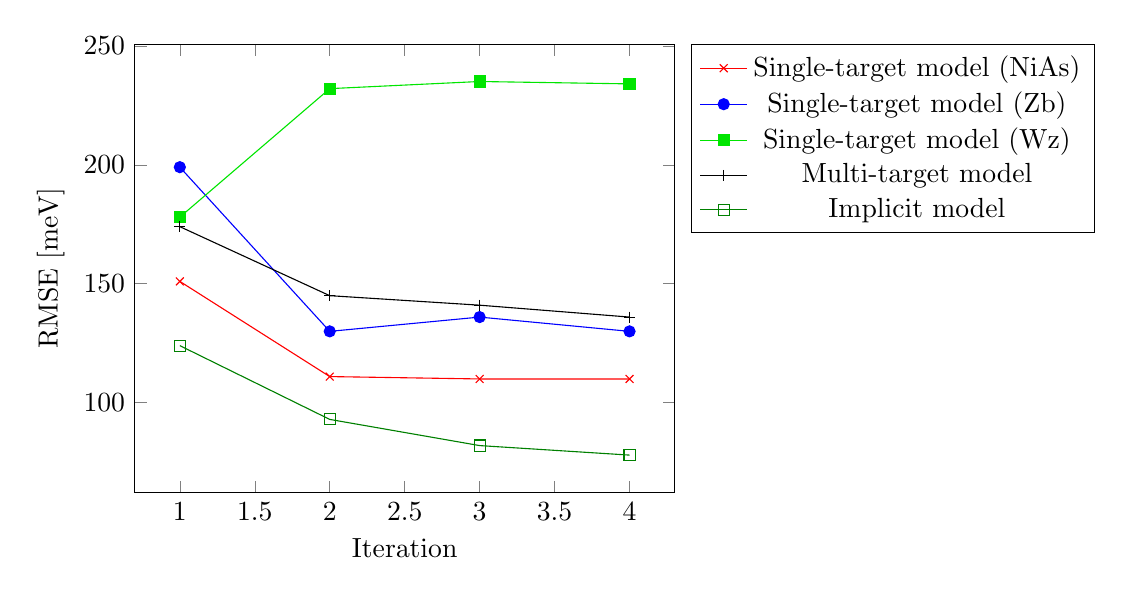
\begin{tikzpicture}
        \begin{axis}[
        xlabel={Iteration},
        ylabel={RMSE [meV]},
        %legend style={at={(1,0.5)}},
        legend pos=outer north east,
        ]
            \addplot[color=red,mark=x] coordinates {
	        (1,   151)
	        (2,   111)
	        (3,   110)
	        (4,   110)
            };
            \addlegendentry{Single-target model (NiAs)}
            \addplot[color=blue,mark=*] coordinates {
	        (1,   199)
	        (2,   130)
	        (3,   136)
	        (4,   130)
            };
            \addlegendentry{Single-target model (Zb)}
            \addplot[color=green!90!black,mark=square*] coordinates {
	        (1,   178)
	        (2,   232)
	        (3,   235)
	        (4,   234)
            };
            \addlegendentry{Single-target model (Wz)}
            \addplot[color=black,mark=+] coordinates {
	        (1,   174)
	        (2,   145)
	        (3,   141)
	        (4,   136)
            };
            \addlegendentry{Multi-target model }
            \addplot[color=green!50!black,mark=square] coordinates {
	        (1,   124)
	        (2,   93)
	        (3,   82)
	        (4,   78)
            };
            \addlegendentry{Implicit model}

            
            
            
        \end{axis}
    \end{tikzpicture}    
    %\fi
    \caption[Error vs. iterations]{Root mean square error as a function of iterations.}
    \label{fig:error_plot}
\end{figure}

\fi


\begin{figure}
    \centering
    %\iffigure
    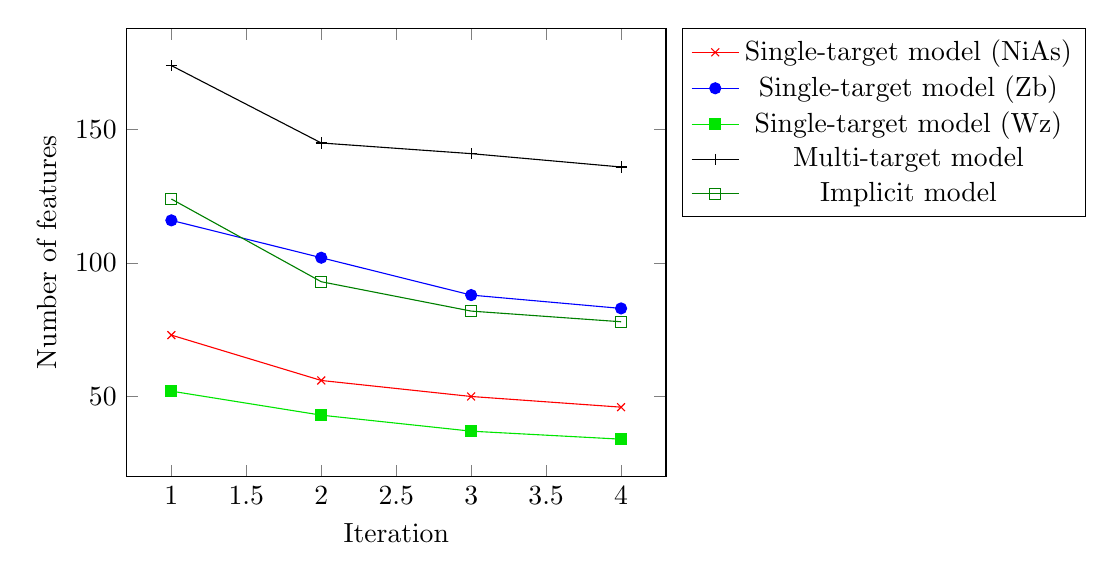
\begin{tikzpicture}
        \begin{axis}[
        xlabel={Iteration},
        ylabel={Number of features},
        %legend style={at={(1,0.5)}},
        legend pos=outer north east,
        ]
            \addplot[color=red,mark=x] coordinates {
	        (1,   73 )
	        (2,   56)
	        (3,   50)
	        (4,   46)
            };
            \addlegendentry{Single-target model (NiAs)}
            \addplot[color=blue,mark=*] coordinates {
	        (1,   116)
	        (2,   102)
	        (3,   88)
	        (4,   83)
            };
            \addlegendentry{Single-target model (Zb)}
            \addplot[color=green!90!black,mark=square*] coordinates {
	        (1,   52 )
	        (2,   43)
	        (3,   37)
	        (4,   34)
            };
            \addlegendentry{Single-target model (Wz)}
            \addplot[color=black,mark=+] coordinates {
	        (1,   174)
	        (2,   145)
	        (3,   141)
	        (4,   136)
            };
            \addlegendentry{Multi-target model }
            \addplot[color=green!50!black,mark=square] coordinates {
	        (1,   124)
	        (2,   93)
	        (3,   82)
	        (4,   78)
            };
            \addlegendentry{Implicit model}

            
            
            
        \end{axis}
    \end{tikzpicture}    
    %\fi
    \caption[Features versus iterations]{Number of features for each model as a function of iterations.}
    \label{fig:error_plot}
\end{figure}


By comparing the \texttt{RMSE} it is evident that the models generally performs best on the NiAs observations. This could tell that the NiAs structure is best suited for the constructed feature vector, but it might as well be due to smaller variance in the test set for the NiAs target values. The maximum error supports this as it also remains the lowest for the NiAs. The maximum error is mostly largest for the Wz structure. This might be due to the potential outlier discussed previously.

Comparing to \emph{Rupp et al.} \citep{rupp} the \texttt{RMSE} of our models are large. As their best was 650 meV per molecule with molecules up to seven atoms, this is less than 100 meV per atom, which is close to the least \texttt{RMSE} that is obtained for the single-target model. There are similarities, but they obtained the results through a kernel ridge regression. Using a Lasso regression, as it is done here, one can obtain smaller \texttt{RMSE} with fewer features on simpler data sets with more highly important features \citep{criticalrole_descriptor}. Partitioning the data in some ways or creating more complex features appropriate for this data set, could help improve the performance of our models. 






